\documentclass[10pt,t,aspectratio=169]{beamer}
%\usetheme{Berkeley}
\usepackage{graphicx}
\usepackage{amsmath}
\usepackage[american]{circuitikz}

% Packages to plot functions
\usepackage{pgfplots}
\pgfplotsset{compat=newest}

\usepackage{multicol}
\usepackage{multirow}
\usepackage{textcomp} % to use \textmu
\usepackage[absolute,overlay]{textpos} % to place floating text boxes with \begin{textblock*}{width}(x,y)
\usepackage{tcolorbox}
\usepackage{colortbl} % allows coloring cells of a table with \cellcolor{blue!25}

\title{Clase 3}
\subtitle{Modelo de bandas de energía}
\author{Dr.-Ing. Juan José Montero Rodríguez}
\subject{Elementos Activos}
\institute{Escuela de Ingeniería Electrónica}
\date{Semestre II-2023}
\titlegraphic{\includegraphics[height=12mm]{figures/logoTEC.pdf}}


\begin{document}

\begin{frame}[t]
\titlepage
\end{frame}



\begin{frame}[t]
    \frametitle{Modelo Atómico de Bohr}

    Fundamentos:
    \begin{itemize}
        \item Principio de cuantización (quantum): niveles discretos de energía.
        \item Electrones pertenecen a un determinado nivel de energía.
        \item Dos electrones no pueden tener los mismos números cuánticos (principio de exclusión Pauli).
    \end{itemize}

    Los electrones existen en niveles de energía caracterizados por el número cuántico principal n $\rightarrow$ relacionado con distancia al núcleo y energía del nivel.

    \centering
    \includegraphics[width=9cm]{./figures/modelo-bohr.jpg}
\end{frame}


\begin{frame}[t]
    \frametitle{Formación de Bandas de Energía}

    \begin{columns}
    
        \begin{column}[]{0.6\textwidth}
        
            Cuando los átomos se aproximan unos a otros, los niveles de energía se desdoblan en niveles de energía muy próximos = bandas de energía
            \begin{itemize}
                \item Bandas: conjunto de niveles de energía electrónicos.
                \item Regiones de probabilidad de encontrar al electrón.
                \item Tres bandas: conducción, valencia y prohibida.
            \end{itemize}

            \vspace{3mm}
            \centering
            \includegraphics[width=0.88\textwidth]{./figures/formacion-bandas-2.jpg}
            
        \end{column}
        
    \begin{column}[]{0.4\textwidth}
    
        \centering
        \includegraphics[width=\textwidth]{./figures/formacion-bandas-1.png}
        \small{La energía de cada electrón no se repite, por lo que, al juntar una gran cantidad de átomos, se forman bandas continuas.}
        
    \end{column}
    
    \end{columns}
    
\end{frame}


\begin{frame}[t]
    \frametitle{Formación de Bandas de Energía}

    \centering
    \includegraphics[width=12cm]{./figures/formacion-bandas-3.jpg}
\end{frame}


\begin{frame}[t]
    \frametitle{Diagrama de Bandas de Energía}

    \begin{itemize}
        \item Diagrama de bandas = energía en función de la posición.
        \item En un diagrama de bandas, $V=E/q$ $\rightarrow$ definido para un electrón con carga negativa.
        \item Estructura básica de un diagrama de bandas de energía de un semiconductor.        
    \end{itemize}

    \begin{figure}[H]
        \centering
        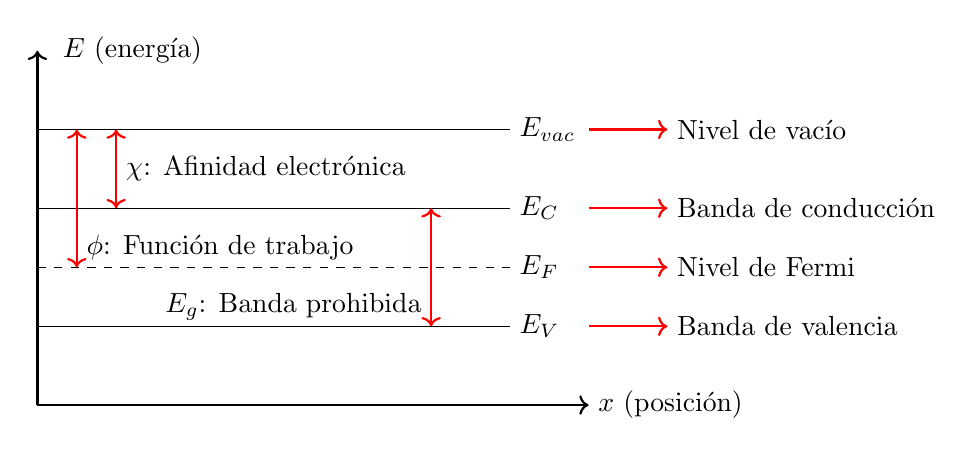
\begin{tikzpicture}
            \draw (0,0) -- (6,0);
            \draw (6,0) node[anchor=west]{$E_{vac}$};
            \draw[thick,->,red] (7,0) -- (8,0);
            \draw (8,0) node[anchor=west]{Nivel de vacío};
            \draw (0,-1) -- (6,-1);
            \draw (6,-1) node[anchor=west]{$E_{C}$};
            \draw[thick,->,red] (7,-1) -- (8,-1);
            \draw (8,-1) node[anchor=west]{Banda de conducción};
            \draw[dashed] (0,-1.75) -- (6,-1.75);
            \draw (6,-1.75) node[anchor=west]{$E_{F}$};
            \draw[thick,->,red] (7,-1.75) -- (8,-1.75);
            \draw (8,-1.75) node[anchor=west]{Nivel de Fermi};
            \draw (0,-2.5) -- (6,-2.5);
            \draw (6,-2.5) node[anchor=west]{$E_{V}$};
            \draw[thick,->,red] (7,-2.5) -- (8,-2.5);
            \draw (8,-2.5) node[anchor=west]{Banda de valencia};
            % Afinidad electronica
            \draw[<->,thick,red] (1,0) -- (1,-1);
            \draw (1,-0.5) node[anchor=west]{$\chi$: Afinidad electrónica};
            % Funcion de trabajo
            \draw[<->,thick,red] (0.5,0) -- (0.5,-1.75);
            \draw (0.5,-1.5) node[anchor=west]{$\phi$: Función de trabajo};
            % Banda prohibida
            \draw[<->,thick,red] (5,-1) -- (5,-2.5);
            \draw (5,-2.25) node[anchor=east]{$E_g$: Banda prohibida};
            % Ejes coordenados
            \draw[thick,->] (0,-3.5) -- (7,-3.5);
            \draw (7,-3.5) node[anchor=west]{$x$ (posición)};
            \draw[thick,->] (0,-3.5) -- (0,1);
            \draw (0.2,1) node[anchor=west]{$E$ (energía)};
        \end{tikzpicture}
    \end{figure}
\end{frame}


\begin{frame}[t]
    \frametitle{Diagrama de Bandas de Energía}

    \textbf{Nivel de vacío:}
    \begin{itemize}
        \item Nivel de referencia (cero).
        \item Nivel de energía a la cual un electrón se ha liberado del material, es decir, no está ligado al sólido.
    \end{itemize}
    
    \textbf{Afinidad electrónica:}
    \begin{itemize}
        \item energía que un electrón en la banda de conducción debe ganar para convertirse en un electrón liberado del material.
        \item Definida para semiconductores.
    \end{itemize}

    \textbf{Función de trabajo:}
    \begin{itemize}
        \item Diferencia de energía entre el nivel de vacío y el nivel de Fermi.
    \end{itemize}
    
    \textbf{Nivel de Fermi intrínseco:}
    \begin{itemize}
        \item Nivel de Fermi intrínseco ubicado aproximadamente en la mitad de la banda prohibida.
        \item Dopado modifica el nivel de Fermi de un material intrínseco de acuerdo con la intensidad y el tipo de impureza.
    \end{itemize}
\end{frame}


\begin{frame}[t]
    \frametitle{Modelo de Bandas de Energía}

    \begin{columns}
        \begin{column}{0.6\textwidth}
            \textbf{Banda de valencia:}
            \begin{itemize}
                \item Nivel de energía más alto que está lleno a 0 K.
                \item Electrones no participan en conducción.
                \item Electrones de esta banda forman enlaces con otros átomos.
            \end{itemize}
            
            \textbf{Banda prohibida:}
            \begin{itemize}
                \item Brecha energética (energy gap).
                \item Banda de estados prohibidos para el electrón.
                \item Energía necesaria para mover un electrón de la banda de valencia a la banda de conducción.
            \end{itemize}
            
            \textbf{Banda de conducción:}
            \begin{itemize}
                \item Nivel de energía separado de la banda de valencia por la banda prohibida.
                \item Electrones participan en conducción.
            \end{itemize}
        \end{column}
        \begin{column}{0.4\textwidth}
            \centering
            \begin{figure}[H]
                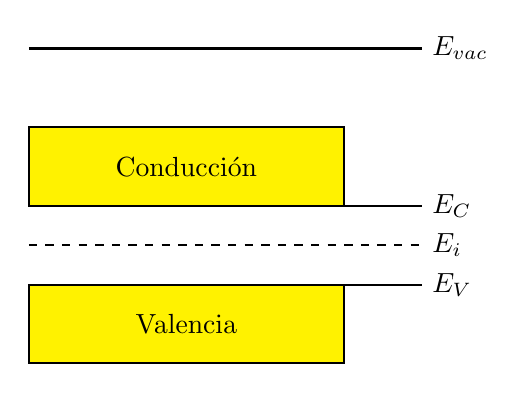
\begin{tikzpicture}
                    % Banda de conduccion
                    \filldraw [thick, fill=yellow, even odd rule] (0,0) rectangle (4,1){};
                    \draw (2,0.5) node[]{Conducción};
                    \draw [thick] (4,0) -- (5,0);
                    \draw (5,0) node[anchor=west]{$E_C$};
                    % Banda de valencia
                    \filldraw [thick, fill=yellow, even odd rule] (0,-1) rectangle (4,-2){};
                    \draw (2,-1.5) node[]{Valencia};
                    \draw [thick] (4,-1) -- (5,-1);
                    \draw (5,-1) node[anchor=west]{$E_V$};
                    % Nivel de vacio
                    \draw [thick] (0,2) -- (5,2);
                    \draw (5,2) node[anchor=west]{$E_{vac}$};
                    % Nivel de Fermi
                    \draw [dashed,thick] (0,-0.5) -- (5,-0.5);
                    \draw (5,-0.5) node[anchor=west]{$E_i$};
                \end{tikzpicture}
            \end{figure}

            \centering
            \small{El diagrama de bandas muestra únicamente los bordes de cada banda.}
        \end{column}
    \end{columns}
\end{frame}


\begin{frame}[t]
    \frametitle{Clasificación de Materiales según Modelo de Bandas de Energía}

    Bandas de energía del material definen propiedades eléctricas, ópticas y térmicas.

    \vspace{3mm}
    Clasificación de acuerdo con propiedades eléctricas:
    
    \vspace{3mm}
    \begin{columns}
        \begin{column}{0.33\textwidth}
            \centering
            \textbf{Conductores}

            \vspace{3mm}
            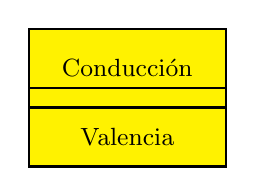
\begin{tikzpicture}
                \filldraw [thick, fill=yellow, even odd rule] (0,0) rectangle (2.5,1){};
                \draw (1.25,0.5) node[]{\small{Conducción}};
                \filldraw [thick, fill=yellow, even odd rule] (0,-0.75) rectangle (2.5,0.25){};
                \draw (1.25,-0.375) node[]{\small{Valencia}};
                \draw [thick] (0,0) -- (2.5,0);
            \end{tikzpicture}

            Ancho de banda prohibida muy pequeño o traslape de bandas

            Cobre, Aluminio, Oro

        \end{column}
        \begin{column}{0.33\textwidth}
            \centering
            \textbf{Semiconductores}

            \vspace{3mm}
            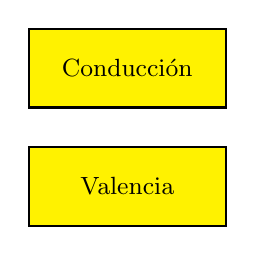
\begin{tikzpicture}
                \filldraw [thick, fill=yellow, even odd rule] (0,0) rectangle (2.5,1){};
                \draw (1.25,0.5) node[]{\small{Conducción}};
                \filldraw [thick, fill=yellow, even odd rule] (0,-1.5) rectangle (2.5,-0.5){};
                \draw (1.25,-1) node[]{\small{Valencia}};
            \end{tikzpicture}

            Banda prohibida = 1-3 eV

            Silicio, Germanio, compuestos como GaAs, InP

        \end{column}
        \begin{column}{0.33\textwidth}
            \centering
            \textbf{Aislantes}
            
            \vspace{3mm}
            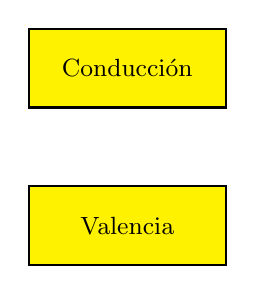
\begin{tikzpicture}
                \filldraw [thick, fill=yellow, even odd rule] (0,0) rectangle (2.5,1){};
                \draw (1.25,0.5) node[]{\small{Conducción}};
                \filldraw [thick, fill=yellow, even odd rule] (0,-2) rectangle (2.5,-1){};
                \draw (1.25,-1.5) node[]{\small{Valencia}};
            \end{tikzpicture}

            Banda prohibida = 8-9 eV

            Diamante, dióxido de silicio (SiO\textsubscript{2}), nitruro de silicio (Si\textsubscript{3}N\textsubscript{4}), dióxido de hafnio (HfO\textsubscript{2})

        \end{column}
    \end{columns}
\end{frame}


\begin{frame}[t]
    \frametitle{Clasificación de Materiales según Conductividad}

    \centering
    \includegraphics[width=10cm]{./figures/conductividad-materiales.pdf}
\end{frame}


\begin{frame}[t]
    \frametitle{Parámetros de Referencia para Materiales Comunes}

    \begin{itemize}
        \item La afinidad electrónica se define para semiconductores.
        \item La banda prohibida es una constante de los semiconductores.
        \item Los metales tienen una función de trabajo constante.
        \item La función de trabajo de los semiconductores depende del dopado.        
    \end{itemize}

    \begin{table}[H]
        \centering\small
        \begin{tabular}{llc}
            \hline Afinidad electrónica & Silicio & 4.05 eV \\
            de semiconductores 	 & Germanio & 4.13 eV \\
	                             & GaAs		& 4.07 eV \\
            \hline Banda prohibida		 & Silicio	& 1.12 eV \\
            de semiconductores	 & Germanio & 0.66 eV \\
			                     & GaAs     & 1.424 eV \\
            \hline Función de trabajo   & Plata	& 4.26 eV \\
            de metales			 & Aluminio & 4.28 eV \\
				                 & Oro		& 5.1 eV \\
                                 & Cromo		& 4.5 eV \\
                                 & Molibdeno	& 4.6 eV \\
                                 & Níquel		& 5.15 eV \\
                                 & Tungsteno	& 4.55 eV \\
            \hline
        \end{tabular}
    \end{table}
\end{frame}


\begin{frame}[t]
    \frametitle{Generación y Recombinación en Silicio Intrínseco}

    \begin{columns}
    
        \begin{column}{0.5\textwidth}
        
            \textbf{Generación:} $G = G_{op} + G_{th}(T) $
            \begin{itemize}
                \item Transición de un electrón de la banda de valencia a la banda de conducción.
                \item Genera un hueco en la banda de valencia.
                \item Creación de pares electrón-hueco
            \end{itemize}
            
            \vspace{3mm}
            \textbf{Recombinación:} $R = k\cdot{}n\cdot{}p$
            \begin{itemize}
                \item Transición de un electrón de la banda de conducción a la banda de valencia.
                \item Elimina un hueco de la banda de valencia.
                \item Eliminación de pares electrón-hueco.
            \end{itemize}

            \vspace{3mm}
            \centering
            La generación y la recombinación ocurren de manera simultánea, hasta que se alcanza una concentración de equilibrio $n_i=10^{10}\ cm^{-3}$
            
        \end{column}
        
        \begin{column}{0.5\textwidth}
        
            \centering
            \includegraphics[height=7cm]{./figures/generacion-recombinacion.pdf}
            
        \end{column}
        
    \end{columns}
    
\end{frame}

\begin{frame}[t]
    \frametitle{Densidad de Estados}

    En cada nivel de energía existe una cierta cantidad de estados disponibles para ser ocupados por los electrones (o huecos).

    \begin{columns}
    
        \begin{column}{0.6\textwidth}
        
            \centering
            \includegraphics[width=9cm]{./figures/dos.png} 
            
        \end{column}
        
        \begin{column}{0.4\textwidth}
        
            $g_c(E)$: densidad de estados en banda de conducción

            \[ g_c(E) = \dfrac{m_n\sqrt{2m_n (E-E_C)}}{\pi^2 h^3} \]

            \flushright con $E>E_C$
                
            \flushleft
            $g_v(E)$: densidad de estados en banda valencia

            \[ g_v(E) = \dfrac{m_p\sqrt{2m_p (E_V-E)}}{\pi^2 h^3} \]

            \flushright con $E\leq{}E_V$
            
        \end{column}
        
    \end{columns}
    
\end{frame}


\begin{frame}[t]
    \frametitle{Distribución de Fermi-Dirac}

    \begin{itemize}
        \item Distribución de Fermi-Dirac: función de densidad de probabilidad con valores entre 0 y 1.
        \item Nivel de Fermi $E_F$: valor de energía en el que la probabilidad de ocupación del estado electrónico es de 50\%
    \end{itemize}

    \begin{columns}
    
        \begin{column}{0.5\textwidth}
        
            \centering
            \includegraphics[width=\textwidth]{./figures/fermi-dirac.pdf}
            
        \end{column}
        
        \begin{column}{0.5\textwidth}
        
            Probabilidad de ocupación de electrones:

            \[ f(E) = \dfrac{1}{1 + e^{\dfrac{E-E_F}{kT}}} \]
        
            \vspace{3mm}
            Probabilidad de ocupación de huecos:
        
            \[ h(E) = 1 - \dfrac{1}{1 + e^{\dfrac{E-E_F}{kT}}} \]
            
        \end{column}
        
    \end{columns}
    
\end{frame}


\begin{frame}[t]
    \frametitle{Distribución de Fermi-Dirac con Distintas Temperaturas}

    La función de Fermi toma distintas formas dependiendo de la temperatura:
    \begin{itemize}
        \item Para T = 0 K, la función toma valores de 0 y 1
        \begin{itemize}
            \item 0 : cero probabilidad de ocupación de electrones
            \item 1 : total probabilidad de ocupación de electrones
        \end{itemize}
        \item Esto significa que por debajo de $E_F$ \textbf{todos} los estados están llenos, y por encima de $E_F$ \textbf{todos} los estados están vacíos
        \item Para $T > 0\ K$, la función se curva y la probabilidad es continua.
    \end{itemize}

    \centering
    \includegraphics[width=9cm]{./figures/fermi-dirac-2.png}
\end{frame}


\begin{frame}[t]
    \frametitle{Portadores en Silicio Intrínseco}

    \centering
    \includegraphics[width=9cm]{./figures/portadores-en-bandas.png}
\end{frame}


\begin{frame}[t]
    \frametitle{Ejemplo: Diagrama de Bandas de Energía}

    Dibuje el diagrama de bandas de energía de los siguientes materiales, indicando los valores numéricos para la función de trabajo, afinidad electrónica, energía de la banda prohibida y la posición del nivel de Fermi.

    \begin{itemize}
        \item Silicio
        \item Oro
        \item Germanio
        \item Tungsteno
    \end{itemize}
\end{frame}


\begin{frame}[t]
    \frametitle{Ejemplo: Nivel de Fermi}
    En una muestra de silicio intrínseco a temperatura ambiente, la probabilidad de ocupación de electrones en un determinado nivel de energía $E_x$ es del 58\%. 

    \begin{itemize}
        \item Determine la posición de ese nivel de energía con respecto al nivel de Fermi intrínseco.
        \item Calcule la probabilidad de ocupación de huecos en ese mismo nivel de energía mencionado.
        \item Dibuje el diagrama de bandas de energía, indicando el nivel energético que tiene la probabilidad de ocupación de electrones propuesta.
        \item Si la muestra de silicio intrínseco está a T = 0 K, indique la probabilidad de ocupación de electrones que existe en el nivel de energía calculado anteriormente.
    \end{itemize}
    
\end{frame}


\begin{frame}{Lecturas recomendadas}
    
\end{frame}

\end{document}
